
%
% 6.869 problem set 3
%
\documentclass[12pt,twoside]{article}

\usepackage{amsmath}
\usepackage{amssymb}
\usepackage{color}
\usepackage{clrscode}
\usepackage[pdftex]{graphicx}

% Cross-references for handout numbers.

% Updated to include SMA course for Fall 2001 -- cel

\newcommand{\name}{}


\usepackage{latexsym}
%\usepackage{bbm}
\usepackage{times,url}
\usepackage{clrscode}

\newcommand{\mitst}[1]{\begin{description}
\item[MIT students:] #1
\end{description}}
\newcommand{\smast}[1]{\begin{description}
\item[SMA students:] #1
\end{description}}

%\newcommand{\collabs}{Professors Srini Devadas, Nancy Lynch and Vinod Vaikuntanathan}
\newcommand{\subj}{6.006}

\newlength{\toppush}
\setlength{\toppush}{2\headheight}
\addtolength{\toppush}{\headsep}

\newcommand{\htitle}[2]{\noindent\vspace*{-\toppush}\newline\parbox{6.5in}
{\textit{6.869 Advances in Computer Vision}\hfill\name\newline
Andrew Moran \hfill #2\newline
\collabs\hfill #1 \vspace*{-.5ex}\newline
\mbox{}\hrulefill\mbox{}}\vspace*{1ex}\mbox{}\newline
\begin{center}{\Large\bf #1}\end{center}}

\newcommand{\handout}[2]{\thispagestyle{empty}
 \markboth{#1}{#1}
 \pagestyle{myheadings}\htitle{#1}{#2}}

\newcommand{\htitlewithouttitle}[2]{\noindent\vspace*{-\toppush}\newline\parbox{6.5in}
{\textit{Introduction to Algorithms}\hfill#2\newline
Massachusetts Institute of Technology \hfill 6.006\newline
%Singapore-MIT Alliance \hfill SMA5503\newline
\profs\hfill Handout #1\vspace*{-.5ex}\newline
\mbox{}\hrulefill\mbox{}}\vspace*{1ex}\mbox{}\newline}

\newcommand{\handoutwithouttitle}[2]{\thispagestyle{empty}
 \markboth{Handout \protect\ref{#1}}{Handout \protect\ref{#1}}
 \pagestyle{myheadings}\htitlewithouttitle{\protect\ref{#1}}{#2}}

\newcommand{\exam}[2]{% parameters: exam name, date
 \thispagestyle{empty}
 \markboth{\subj\ #1\hspace{1in}Name\hrulefill\ \ }%
          {\subj\ #1\hspace{1in}Name\hrulefill\ \ }
 \pagestyle{myheadings}\examtitle{#1}{#2}
 \renewcommand{\theproblem}{Problem \arabic{problemnum}}
}
\newcommand{\examsolutions}[3]{% parameters: handout, exam name, date
 \thispagestyle{empty}
 \markboth{Handout \protect\ref{#1}: #2}{Handout \protect\ref{#1}: #2}
% \pagestyle{myheadings}\htitle{\protect\ref{#1}}{#2}{#3}
 \pagestyle{myheadings}\examsolutionstitle{\protect\ref{#1}} {#2}{#3}
 \renewcommand{\theproblem}{Problem \arabic{problemnum}}
}
\newcommand{\examsolutionstitle}[3]{\noindent\vspace*{-\toppush}\newline\parbox{6.5in}
{\textit{Introduction to Algorithms}\hfill#3\newline
Massachusetts Institute of Technology \hfill 6.006\newline
%Singapore-MIT Alliance \hfill SMA5503\newline
\profs\hfill Handout #1\vspace*{-.5ex}\newline
\mbox{}\hrulefill\mbox{}}\vspace*{1ex}\mbox{}\newline
\begin{center}{\Large\bf #2}\end{center}}

\newcommand{\takehomeexam}[2]{% parameters: exam name, date
 \thispagestyle{empty}
 \markboth{\subj\ #1\hfill}{\subj\ #1\hfill}
 \pagestyle{myheadings}\examtitle{#1}{#2}
 \renewcommand{\theproblem}{Problem \arabic{problemnum}}
}

\makeatletter
\newcommand{\exambooklet}[2]{% parameters: exam name, date
 \thispagestyle{empty}
 \markboth{\subj\ #1}{\subj\ #1}
 \pagestyle{myheadings}\examtitle{#1}{#2}
 \renewcommand{\theproblem}{Problem \arabic{problemnum}}
 \renewcommand{\problem}{\newpage
 \item \let\@currentlabel=\theproblem
 \markboth{\subj\ #1, \theproblem}{\subj\ #1, \theproblem}}
}
\makeatother


\newcommand{\examtitle}[2]{\noindent\vspace*{-\toppush}\newline\parbox{6.5in}
{\textit{Introduction to Algorithms}\hfill#2\newline
Massachusetts Institute of Technology \hfill 6.006 Spring 2014\newline
%Singapore-MIT Alliance \hfill SMA5503\newline
\profs\hfill #1\vspace*{-.5ex}\newline
\mbox{}\hrulefill\mbox{}}\vspace*{1ex}\mbox{}\newline
\begin{center}{\Large\bf #1}\end{center}}

\newcommand{\grader}[1]{\hspace{1cm}\textsf{\textbf{#1}}\hspace{1cm}}

\newcommand{\points}[1]{[#1 points]\ }
\newcommand{\parts}[1]
{
  \ifnum#1=1
  (1 part)
  \else
  (#1 parts)
  \fi
  \ 
}

\newcommand{\bparts}{\begin{problemparts}}
\newcommand{\eparts}{\end{problemparts}}
\newcommand{\ppart}{\problempart}

%\newcommand{\lg} {lg\ }

\setlength{\oddsidemargin}{0pt}
\setlength{\evensidemargin}{0pt}
\setlength{\textwidth}{6.5in}
\setlength{\topmargin}{0in}
\setlength{\textheight}{8.5in}


\newcommand{\Spawn}{{\bf spawn} }
\newcommand{\Sync}{{\bf sync}}

\renewcommand{\cases}[1]{\left\{ \begin{array}{ll}#1\end{array}\right.}
\newcommand{\cif}[1]{\mbox{if $#1$}}
\newcommand{\cwhen}[1]{\mbox{when $#1$}}

\newcounter{problemnum}
\newcommand{\theproblem}{Problem \theproblemsetnum-\arabic{problemnum}}
\newenvironment{problems}{
        \begin{list}{{\bf \theproblem. \hspace*{0.5em}}}
        {\setlength{\leftmargin}{0em}
         \setlength{\rightmargin}{0em}
         \setlength{\labelwidth}{0em}
         \setlength{\labelsep}{0em}
         \usecounter{problemnum}}}{\end{list}}
\makeatletter
\newcommand{\problem}[1][{}]{\item \let\@currentlabel=\theproblem \textbf{#1}}
\makeatother

\newcounter{problempartnum}[problemnum]
\newenvironment{problemparts}{
        \begin{list}{{\bf (\alph{problempartnum})}}
        {\setlength{\leftmargin}{2.5em}
         \setlength{\rightmargin}{2.5em}
         \setlength{\labelsep}{0.5em}}}{\end{list}}
\newcommand{\problempart}{\addtocounter{problempartnum}{1}\item}

\newenvironment{truefalseproblemparts}{
        \begin{list}{{\bf (\alph{problempartnum})\ \ \ T\ \ F\hfil}}
        {\setlength{\leftmargin}{4.5em}
         \setlength{\rightmargin}{2.5em}
         \setlength{\labelsep}{0.5em}
         \setlength{\labelwidth}{4.5em}}}{\end{list}}

\newcounter{exercisenum}
\newcommand{\theexercise}{Exercise \theproblemsetnum-\arabic{exercisenum}}
\newenvironment{exercises}{
        \begin{list}{{\bf \theexercise. \hspace*{0.5em}}}
        {\setlength{\leftmargin}{0em}
         \setlength{\rightmargin}{0em}
         \setlength{\labelwidth}{0em}
         \setlength{\labelsep}{0em}
        \usecounter{exercisenum}}}{\end{list}}
\makeatletter
\newcommand{\exercise}{\item \let\@currentlabel=\theexercise}
\makeatother

\newcounter{exercisepartnum}[exercisenum]
%\newcommand{\problem}[1]{\medskip\mbox{}\newline\noindent{\bf Problem #1.}\hspace*{1em}}
%\newcommand{\exercise}[1]{\medskip\mbox{}\newline\noindent{\bf Exercise #1.}\hspace*{1em}}

\newenvironment{exerciseparts}{
        \begin{list}{{\bf (\alph{exercisepartnum})}}
        {\setlength{\leftmargin}{2.5em}
         \setlength{\rightmargin}{2.5em}
         \setlength{\labelsep}{0.5em}}}{\end{list}}
\newcommand{\exercisepart}{\addtocounter{exercisepartnum}{1}\item}


% Macros to make captions print with small type and 'Figure xx' in bold.
\makeatletter
\def\fnum@figure{{\bf Figure \thefigure}}
\def\fnum@table{{\bf Table \thetable}}
\let\@mycaption\caption
%\long\def\@mycaption#1[#2]#3{\addcontentsline{\csname
%  ext@#1\endcsname}{#1}{\protect\numberline{\csname 
%  the#1\endcsname}{\ignorespaces #2}}\par
%  \begingroup
%    \@parboxrestore
%    \small
%    \@makecaption{\csname fnum@#1\endcsname}{\ignorespaces #3}\par
%  \endgroup}
%\def\mycaption{\refstepcounter\@captype \@dblarg{\@mycaption\@captype}}
%\makeatother
\let\mycaption\caption
%\newcommand{\figcaption}[1]{\mycaption[]{#1}}

\newcounter{totalcaptions}
\newcounter{totalart}

\newcommand{\figcaption}[1]{\addtocounter{totalcaptions}{1}\caption[]{#1}}

% \psfigures determines what to do for figures:
%       0 means just leave vertical space
%       1 means put a vertical rule and the figure name
%       2 means insert the PostScript version of the figure
%       3 means put the figure name flush left or right
\newcommand{\psfigures}{0}
\newcommand{\spacefigures}{\renewcommand{\psfigures}{0}}
\newcommand{\rulefigures}{\renewcommand{\psfigures}{1}}
\newcommand{\macfigures}{\renewcommand{\psfigures}{2}}
\newcommand{\namefigures}{\renewcommand{\psfigures}{3}}

\newcommand{\figpart}[1]{{\bf (#1)}\nolinebreak[2]\relax}
\newcommand{\figparts}[2]{{\bf (#1)--(#2)}\nolinebreak[2]\relax}


\macfigures     % STATE

% When calling \figspace, make sure to leave a blank line afterward!!
% \widefigspace is for figures that are more than 28pc wide.
\newlength{\halffigspace} \newlength{\wholefigspace}
\newlength{\figruleheight} \newlength{\figgap}
\newcommand{\setfiglengths}{\ifnum\psfigures=1\setlength{\figruleheight}{\hruleheight}\setlength{\figgap}{1em}\else\setlength{\figruleheight}{0pt}\setlength{\figgap}{0em}\fi}
\newcommand{\figspace}[2]{\ifnum\psfigures=0\leavefigspace{#1}\else%
\setfiglengths%
\setlength{\wholefigspace}{#1}\setlength{\halffigspace}{.5\wholefigspace}%
\rule[-\halffigspace]{\figruleheight}{\wholefigspace}\hspace{\figgap}#2\fi}
\newlength{\widefigspacewidth}
% Make \widefigspace put the figure flush right on the text page.
\newcommand{\widefigspace}[2]{
\ifnum\psfigures=0\leavefigspace{#1}\else%
\setfiglengths%
\setlength{\widefigspacewidth}{28pc}%
\addtolength{\widefigspacewidth}{-\figruleheight}%
\setlength{\wholefigspace}{#1}\setlength{\halffigspace}{.5\wholefigspace}%
\makebox[\widefigspacewidth][r]{#2\hspace{\figgap}}\rule[-\halffigspace]{\figruleheight}{\wholefigspace}\fi}
\newcommand{\leavefigspace}[1]{\setlength{\wholefigspace}{#1}\setlength{\halffigspace}{.5\wholefigspace}\rule[-\halffigspace]{0em}{\wholefigspace}}

% Commands for including figures with macpsfig.
% To use these commands, documentstyle ``macpsfig'' must be specified.
\newlength{\macfigfill}
\makeatother
\newlength{\bbx}
\newlength{\bby}
\newcommand{\macfigure}[5]{\addtocounter{totalart}{1}
\ifnum\psfigures=2%
\setlength{\bbx}{#2}\addtolength{\bbx}{#4}%
\setlength{\bby}{#3}\addtolength{\bby}{#5}%
\begin{flushleft}
\ifdim#4>28pc\setlength{\macfigfill}{#4}\addtolength{\macfigfill}{-28pc}\hspace*{-\macfigfill}\fi%
\mbox{\psfig{figure=./#1.ps,%
bbllx=#2,bblly=#3,bburx=\bbx,bbury=\bby}}
\end{flushleft}%
\else\ifdim#4>28pc\widefigspace{#5}{#1}\else\figspace{#5}{#1}\fi\fi}
\makeatletter

\newlength{\savearraycolsep}
\newcommand{\narrowarray}[1]{\setlength{\savearraycolsep}{\arraycolsep}\setlength{\arraycolsep}{#1\arraycolsep}}
\newcommand{\normalarray}{\setlength{\arraycolsep}{\savearraycolsep}}

\newcommand{\hint}{{\em Hint:\ }}

% Macros from /th/u/clr/mac.tex

\newcommand{\set}[1]{\left\{ #1 \right\}}
\newcommand{\abs}[1]{\left| #1\right|}
\newcommand{\card}[1]{\left| #1\right|}
\newcommand{\floor}[1]{\left\lfloor #1 \right\rfloor}
\newcommand{\ceil}[1]{\left\lceil #1 \right\rceil}
\newcommand{\ang}[1]{\ifmmode{\left\langle #1 \right\rangle}
   \else{$\left\langle${#1}$\right\rangle$}\fi}
        % the \if allows use outside mathmode,
        % but will swallow following space there!
\newcommand{\paren}[1]{\left( #1 \right)}
\newcommand{\bracket}[1]{\left[ #1 \right]}
\newcommand{\prob}[1]{\Pr\left\{ #1 \right\}}
\newcommand{\Var}{\mathop{\rm Var}\nolimits}
\newcommand{\expect}[1]{{\rm E}\left[ #1 \right]}
\newcommand{\expectsq}[1]{{\rm E}^2\left[ #1 \right]}
\newcommand{\variance}[1]{{\rm Var}\left[ #1 \right]}
\renewcommand{\choose}[2]{{{#1}\atopwithdelims(){#2}}}
\def\pmod#1{\allowbreak\mkern12mu({\rm mod}\,\,#1)}
\newcommand{\matx}[2]{\left(\begin{array}{*{#1}{c}}#2\end{array}\right)}
\newcommand{\Adj}{\mathop{\rm Adj}\nolimits}

\newtheorem{theorem}{Theorem}
\newtheorem{lemma}[theorem]{Lemma}
\newtheorem{corollary}[theorem]{Corollary}
\newtheorem{xample}{Example}
\newtheorem{definition}{Definition}
\newenvironment{example}{\begin{xample}\rm}{\end{xample}}
\newcommand{\proof}{\noindent{\em Proof.}\hspace{1em}}
\def\squarebox#1{\hbox to #1{\hfill\vbox to #1{\vfill}}}
\newcommand{\qedbox}{\vbox{\hrule\hbox{\vrule\squarebox{.667em}\vrule}\hrule}}
\newcommand{\qed}{\nopagebreak\mbox{}\hfill\qedbox\smallskip}
\newcommand{\eqnref}[1]{(\protect\ref{#1})}

%%\newcommand{\twodots}{\mathinner{\ldotp\ldotp}}
\newcommand{\transpose}{^{\mbox{\scriptsize \sf T}}}
\newcommand{\amortized}[1]{\widehat{#1}}

\newcommand{\punt}[1]{}

%%% command for putting definitions into boldface
% New style for defined terms, as of 2/23/88, redefined by THC.
\newcommand{\defn}[1]{{\boldmath\textit{\textbf{#1}}}}
\newcommand{\defi}[1]{{\textit{\textbf{#1\/}}}}

\newcommand{\red}{\leq_{\rm P}}
\newcommand{\lang}[1]{%
\ifmmode\mathord{\mathcode`-="702D\rm#1\mathcode`\-="2200}\else{\rm#1}\fi}

%\newcommand{\ckt}[1]{\ifmmode\mathord{\mathcode`-="702D\sc #1\mathcode`\-="2200}\else$\mathord{\mathcode`-="702D\sc #1\mathcode`\-="2200}$\fi}
\newcommand{\ckt}[1]{\ifmmode \sc #1\else$\sc #1$\fi}

%% Margin notes - use \notesfalse to turn off notes.
\setlength{\marginparwidth}{0.6in}
\reversemarginpar
\newif\ifnotes
\notestrue
\newcommand{\longnote}[1]{
  \ifnotes
    {\medskip\noindent Note: \marginpar[\hfill$\Longrightarrow$]
      {$\Longleftarrow$}{#1}\medskip}
  \fi}
\newcommand{\note}[1]{
  \ifnotes
    {\marginpar{\tiny \raggedright{#1}}}
  \fi}


\newcommand{\reals}{\mathbbm{R}}
\newcommand{\integers}{\mathbbm{Z}}
\newcommand{\naturals}{\mathbbm{N}}
\newcommand{\rationals}{\mathbbm{Q}}
\newcommand{\complex}{\mathbbm{C}}

\newcommand{\oldreals}{{\bf R}}
\newcommand{\oldintegers}{{\bf Z}}
\newcommand{\oldnaturals}{{\bf N}}
\newcommand{\oldrationals}{{\bf Q}}
\newcommand{\oldcomplex}{{\bf C}}

\newcommand{\w}{\omega}                 %% for fft chapter

\newenvironment{closeitemize}{\begin{list}
{$\bullet$}
{\setlength{\itemsep}{-0.2\baselineskip}
\setlength{\topsep}{0.2\baselineskip}
\setlength{\parskip}{0pt}}}
{\end{list}}

% These are necessary within a {problems} environment in order to restore
% the default separation between bullets and items.
\newenvironment{normalitemize}{\setlength{\labelsep}{0.5em}\begin{itemize}}
                              {\end{itemize}}
\newenvironment{normalenumerate}{\setlength{\labelsep}{0.5em}\begin{enumerate}}
                                {\end{enumerate}}

%\def\eqref#1{Equation~(\ref{eq:#1})}
%\newcommand{\eqref}[1]{Equation (\ref{eq:#1})}
\newcommand{\eqreftwo}[2]{Equations (\ref{eq:#1}) and~(\ref{eq:#2})}
\newcommand{\ineqref}[1]{Inequality~(\ref{ineq:#1})}
\newcommand{\ineqreftwo}[2]{Inequalities (\ref{ineq:#1}) and~(\ref{ineq:#2})}

\newcommand{\figref}[1]{Figure~\ref{fig:#1}}
\newcommand{\figreftwo}[2]{Figures \ref{fig:#1} and~\ref{fig:#2}}

\newcommand{\liref}[1]{line~\ref{li:#1}}
\newcommand{\Liref}[1]{Line~\ref{li:#1}}
\newcommand{\lirefs}[2]{lines \ref{li:#1}--\ref{li:#2}}
\newcommand{\Lirefs}[2]{Lines \ref{li:#1}--\ref{li:#2}}
\newcommand{\lireftwo}[2]{lines \ref{li:#1} and~\ref{li:#2}}
\newcommand{\lirefthree}[3]{lines \ref{li:#1}, \ref{li:#2}, and~\ref{li:#3}}

\newcommand{\lemlabel}[1]{\label{lem:#1}}
\newcommand{\lemref}[1]{Lemma~\ref{lem:#1}} 

\newcommand{\exref}[1]{Exercise~\ref{ex:#1}}

\newcommand{\handref}[1]{Handout~\ref{#1}}

\newcommand{\defref}[1]{Definition~\ref{def:#1}}

% (1997.8.16: Victor Luchangco)
% Modified \hlabel to only get date and to use handouts counter for number.
%   New \handout and \handoutwithouttitle commands in newmac.tex use this.
%   The date is referenced by <label>-date.
%   (Retained old definition as \hlabelold.)
%   Defined \hforcelabel to use an argument instead of the handouts counter.

\newcounter{handouts}
\setcounter{handouts}{0}

\newcommand{\hlabel}[2]{%
\stepcounter{handouts}
{\edef\next{\write\@auxout{\string\newlabel{#1}{{\arabic{handouts}}{0}}}}\next}
\write\@auxout{\string\newlabel{#1-date}{{#2}{0}}}
}

\newcommand{\hforcelabel}[3]{%          Does not step handouts counter.
\write\@auxout{\string\newlabel{#1}{{#2}{0}}}
\write\@auxout{\string\newlabel{#1-date}{{#3}{0}}}}


% less ugly underscore
% --juang, 2008 oct 05
\renewcommand{\_}{\vrule height 0 pt depth 0.4 pt width 0.5 em \,}


\setlength{\oddsidemargin}{0pt}
\setlength{\evensidemargin}{0pt}
\setlength{\textwidth}{6.5in}
\setlength{\topmargin}{0in}
\setlength{\textheight}{8.5in}

\newcommand{\theproblemsetnum}{3}
\newcommand{\partaduedate}{Sept 25, 2014 (1:00pm)}
\newcommand{\collabs}{Collaborators: None}
\newcommand{\tabUnit}{3ex}
\newcommand{\tabT}{\hspace*{\tabUnit}}

\title{6.869 PSET 3}

\begin{document}

\handout{Problem Set \theproblemsetnum}{Sept 25, 2014 (1:00pm)}
\tabT Resources with corresponding images and code are on Stellar under \texttt{andrewmo@mit.edu}.  The files are in the \texttt{pset3.zip} folder.  To reproduce the below figures, run \texttt{pset3main.m}.


\section*{Problem 1}
\tabT \textbf{(A)} The data provided is sampled at wavelengths $[360: 5: 730]nm$. A set of primaries $p_i(\lambda)$ is associated with a set of color matching functions $c_i(\lambda)$ if
\newline
\newline
\tabT\tabT\tabT\tabT\tabT\tabT\tabT\tabT\tabT$\sum_{i} (p_i(\lambda) \sum_{\lambda_{i}} c_i(\lambda_{1}) s(\lambda_{1}))$
\newline

\tabT \textbf{(i)} To compute the color matching functions asociated with those specified by the RGB primaries, we use the provided transformation matrix $T$ on the XYZ color function matrix $C_{XYZ}$.  Therefore, $C_{RGB} = T \times C_{XYZ}$.

\DeclareGraphicsExtensions{.pdf,.png,.jpg}
    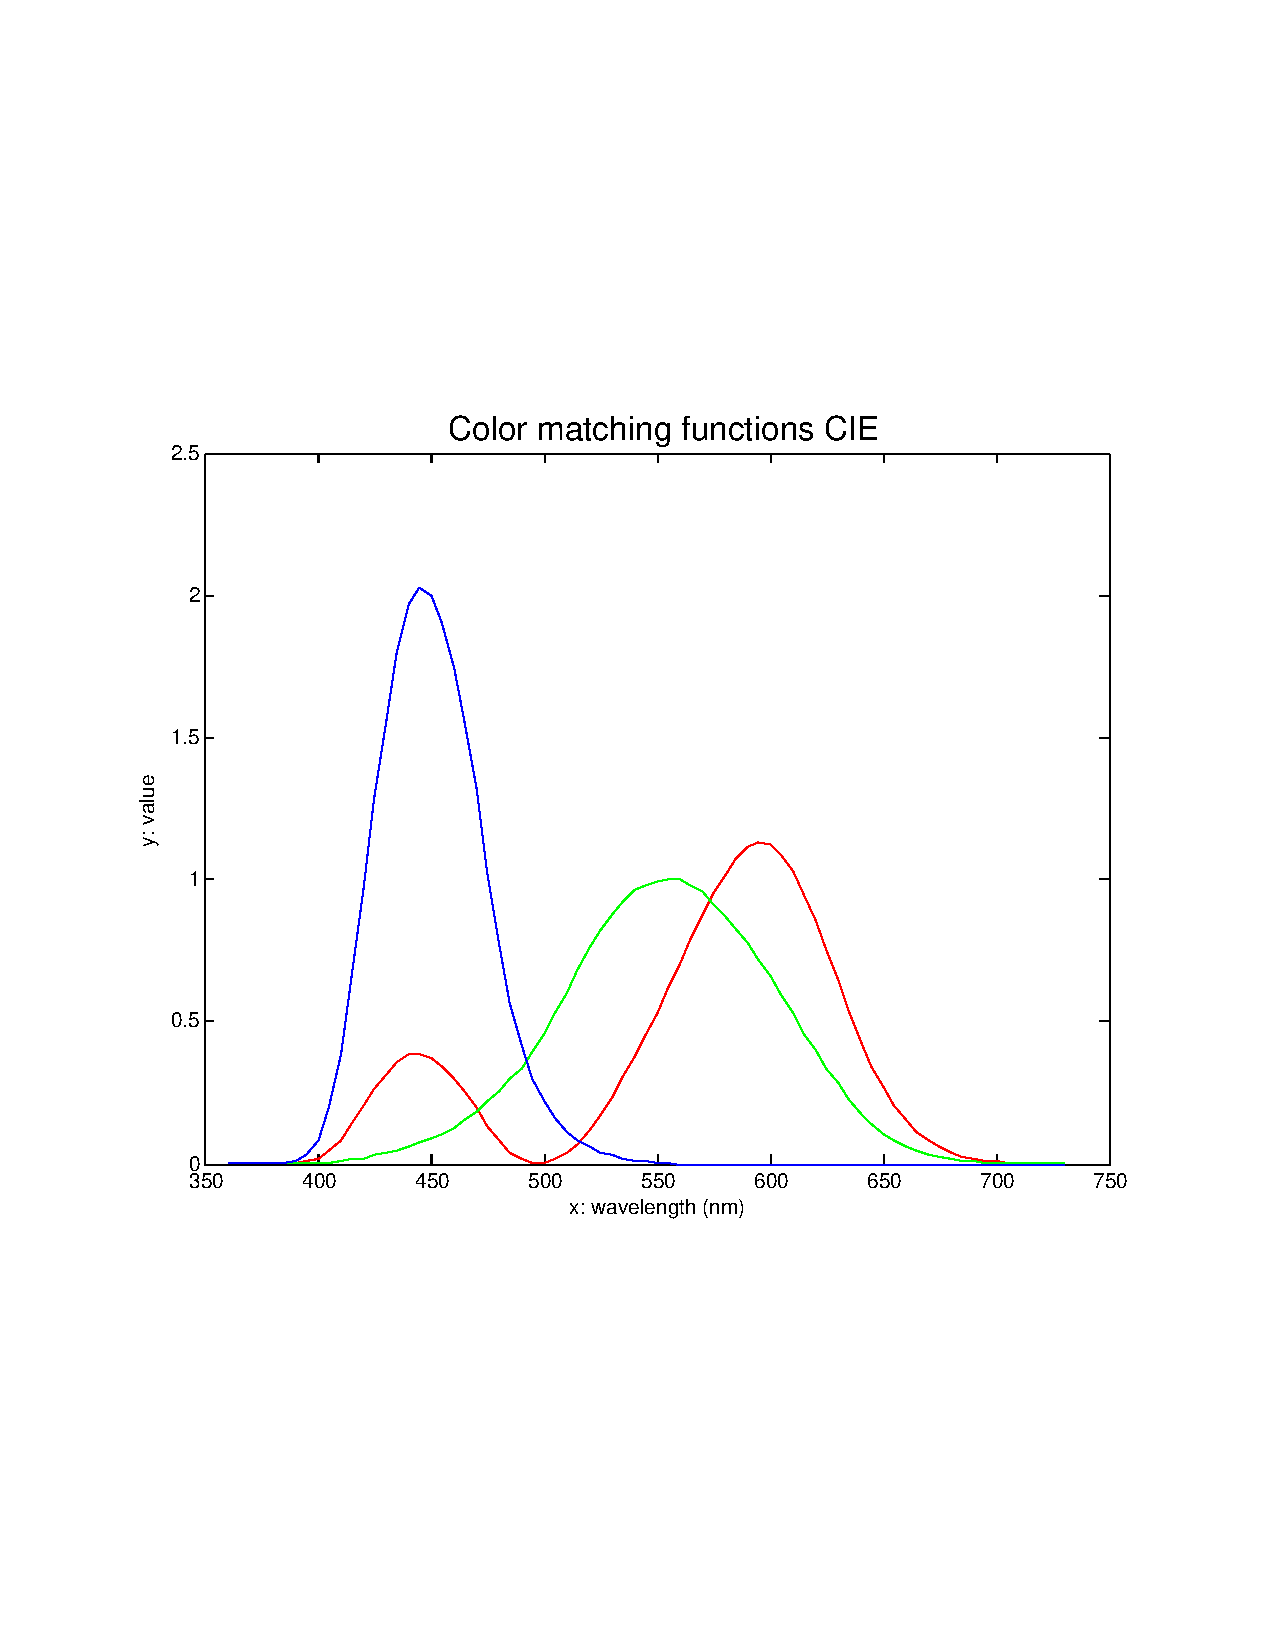
\includegraphics[width = 200pt, trim = 50pt 50pt 50pt 50pt, clip]{C_CIE} 
    \tabT\tabT 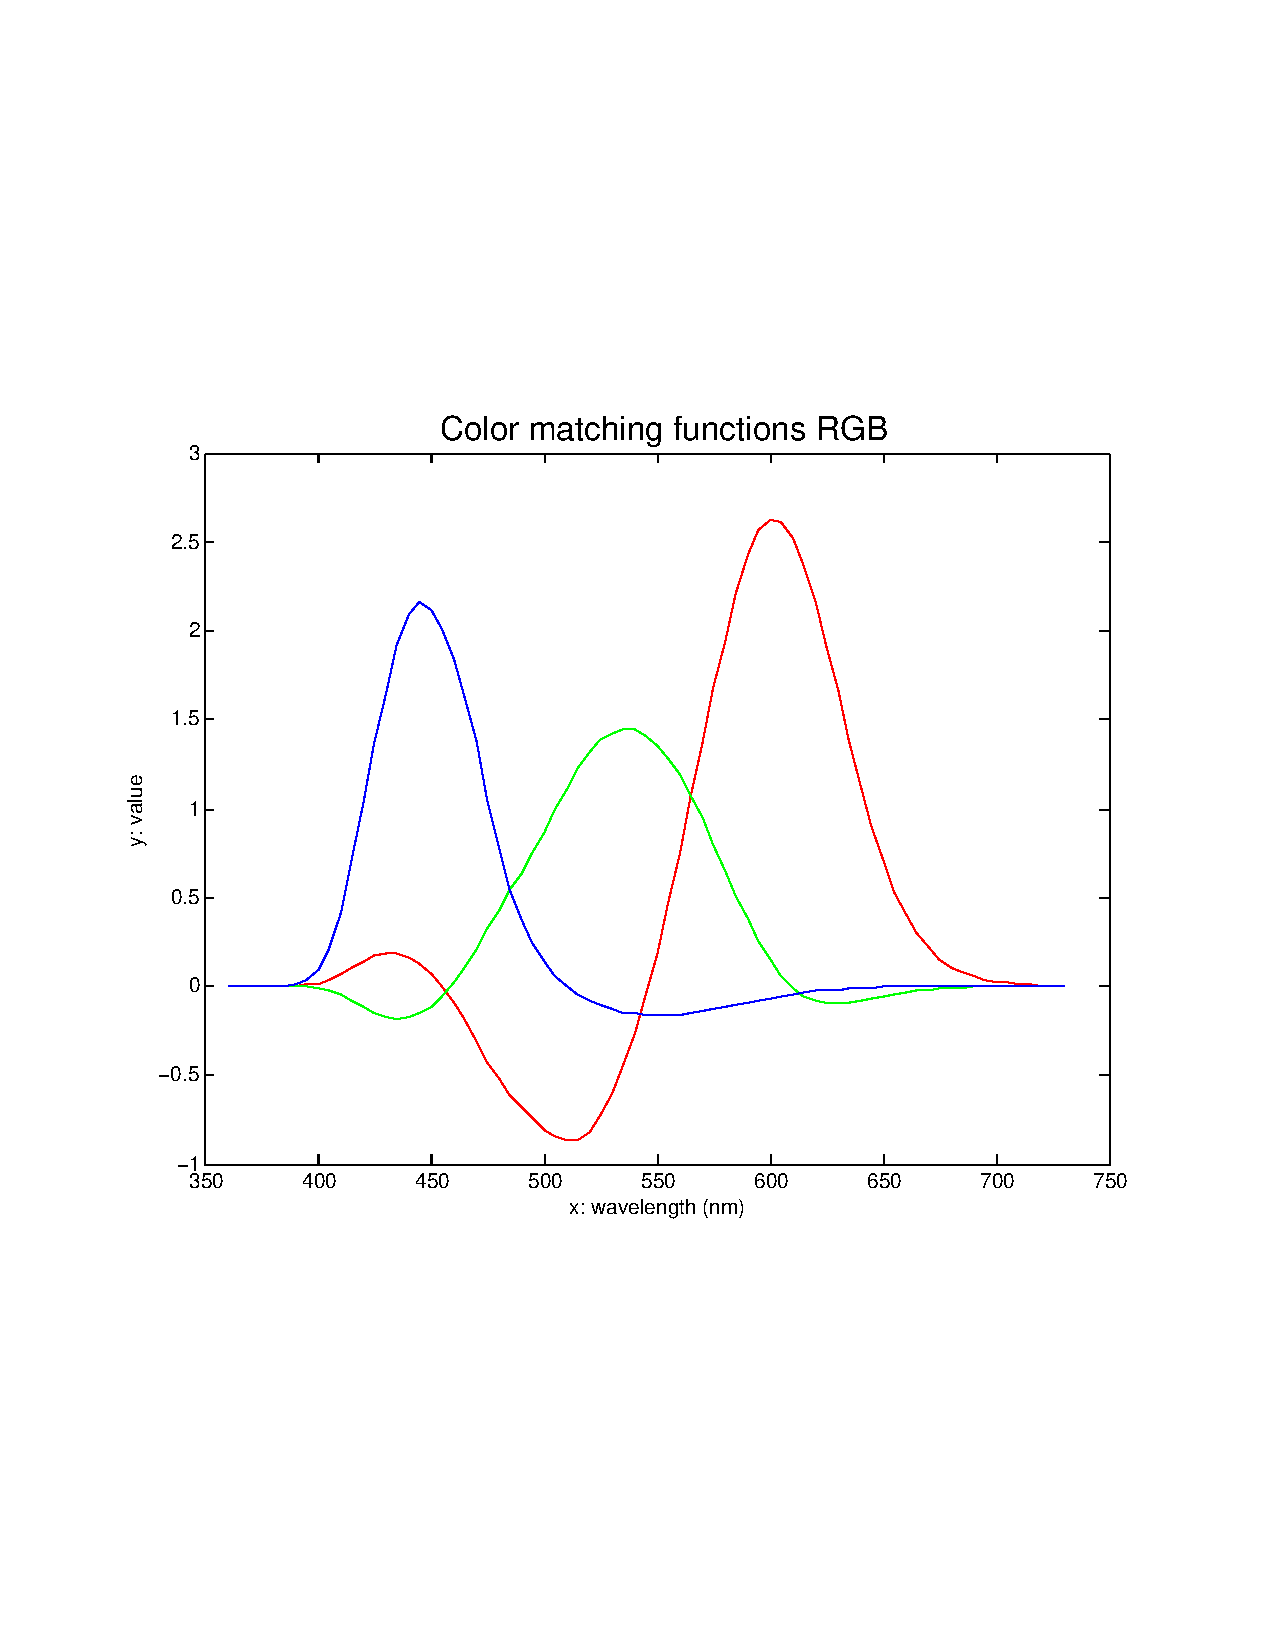
\includegraphics[width = 200pt, trim = 50pt 50pt 50pt 50pt, clip]{C_RGB}

For the XYZ colorspace, notice how none of the color mathcing functions are negative.  This is because XYZ space basically normalizes the RGB space.
For the RGB colorpsace, some of the color matching functions are negative.  This means that some primaries need to be added to the sample space in addtion to combining the primaries in order to get a correct color matching.
\newline



For the following problems, we need to find the primary light spectra associated with the color function matrices.
\newline
\tabT\tabT\tabT\tabT\tabT\tabT\tabT\tabT\tabT$s = Ct$ \newline
\tabT\tabT\tabT\tabT\tabT\tabT\tabT\tabT\tabT$t = Ps$ \newline
\tabT\tabT\tabT\tabT\tabT\tabT\tabT\tabT\tabT$PCs = s$ \newline
\tabT\tabT\tabT\tabT\tabT\tabT\tabT\tabT\tabT$PC = I$ \newline
\tabT\tabT\tabT\tabT\tabT\tabT\tabT\tabT\tabT$P = C^{-1}$ \newline
\newline
In other words, the primary light spectra $P$ is the psedo-inverse of the color function matrix $C$ since $C$ can be an underdetermined system and $PC = I$.  Below are the light spectras for RGB (\textbf{a.ii}) and XYZ (\textbf{a.iii}), respectively.
\newline
\DeclareGraphicsExtensions{.pdf,.png,.jpg}
\begin{tabular}{ c c }
 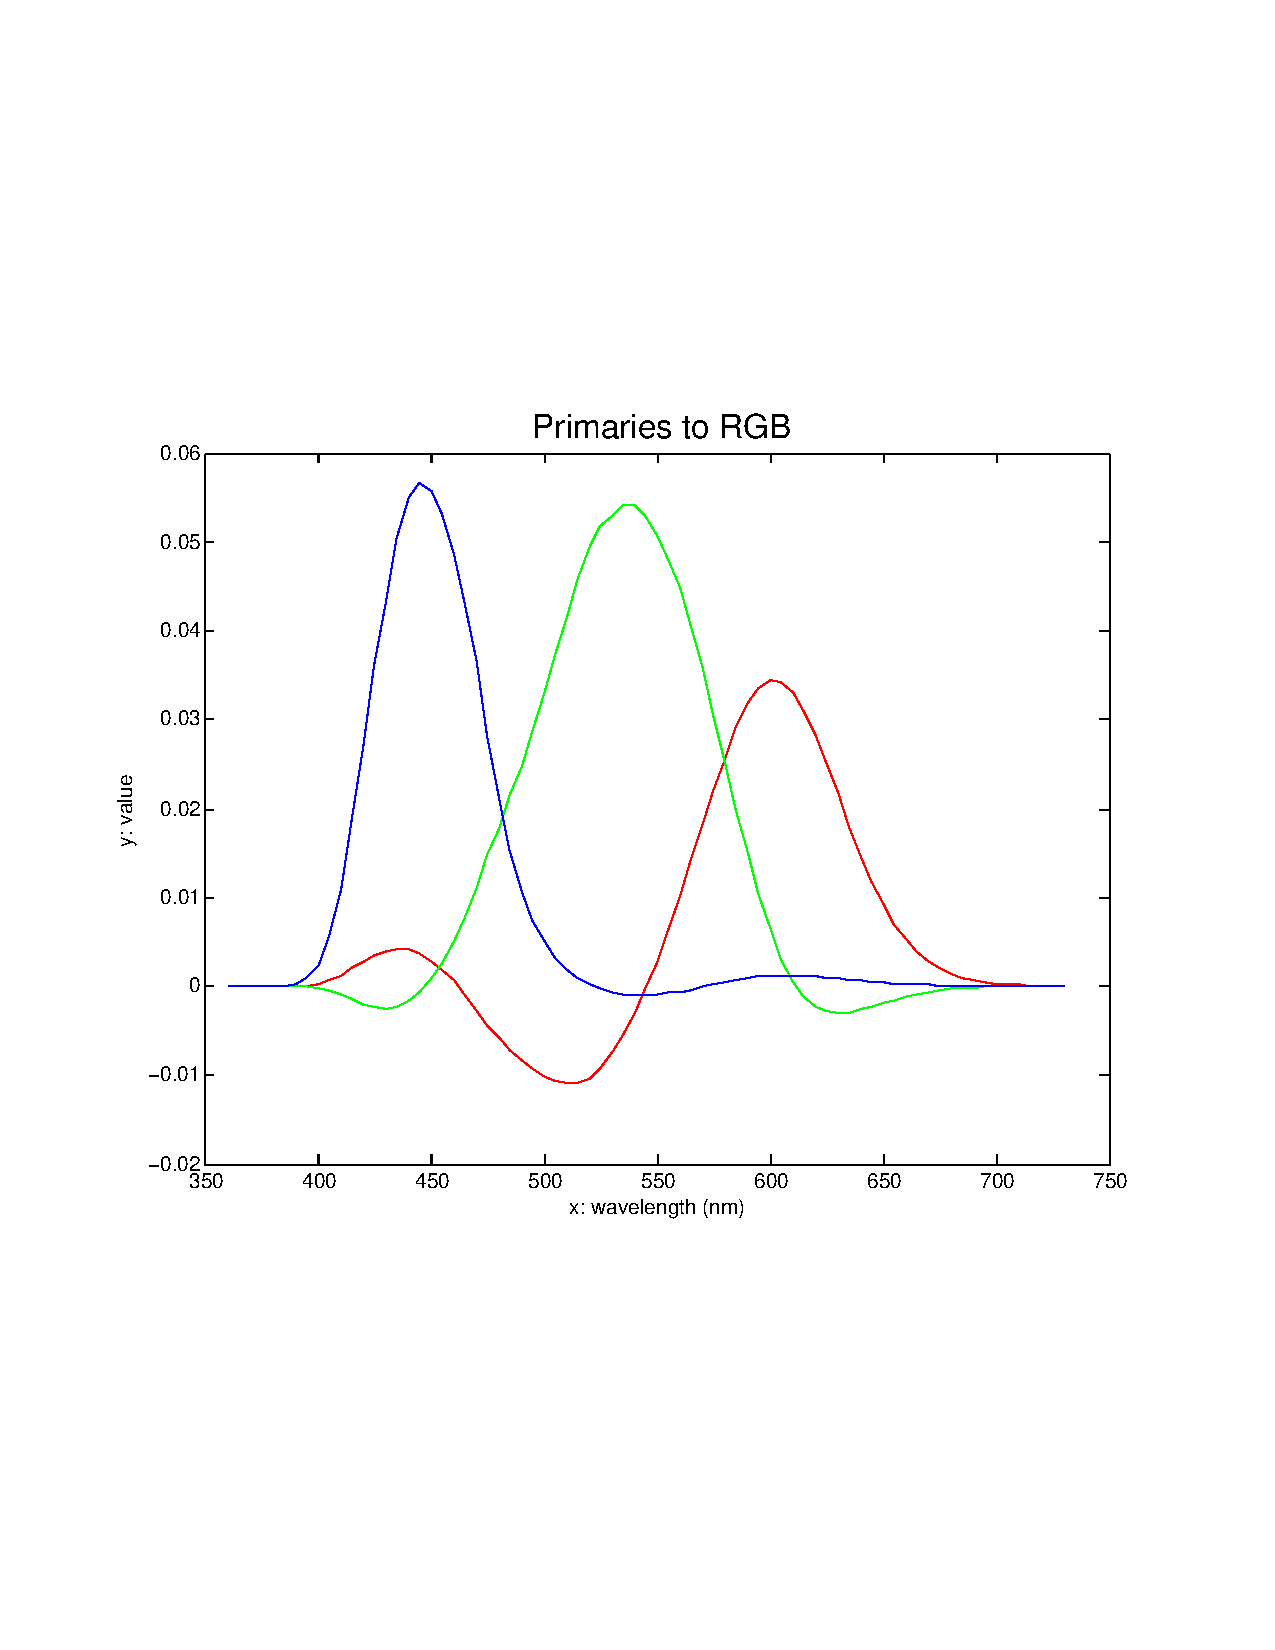
\includegraphics[width = 200pt, trim = 50pt 50pt 50pt 50pt, clip]{P_RGB} 
 & 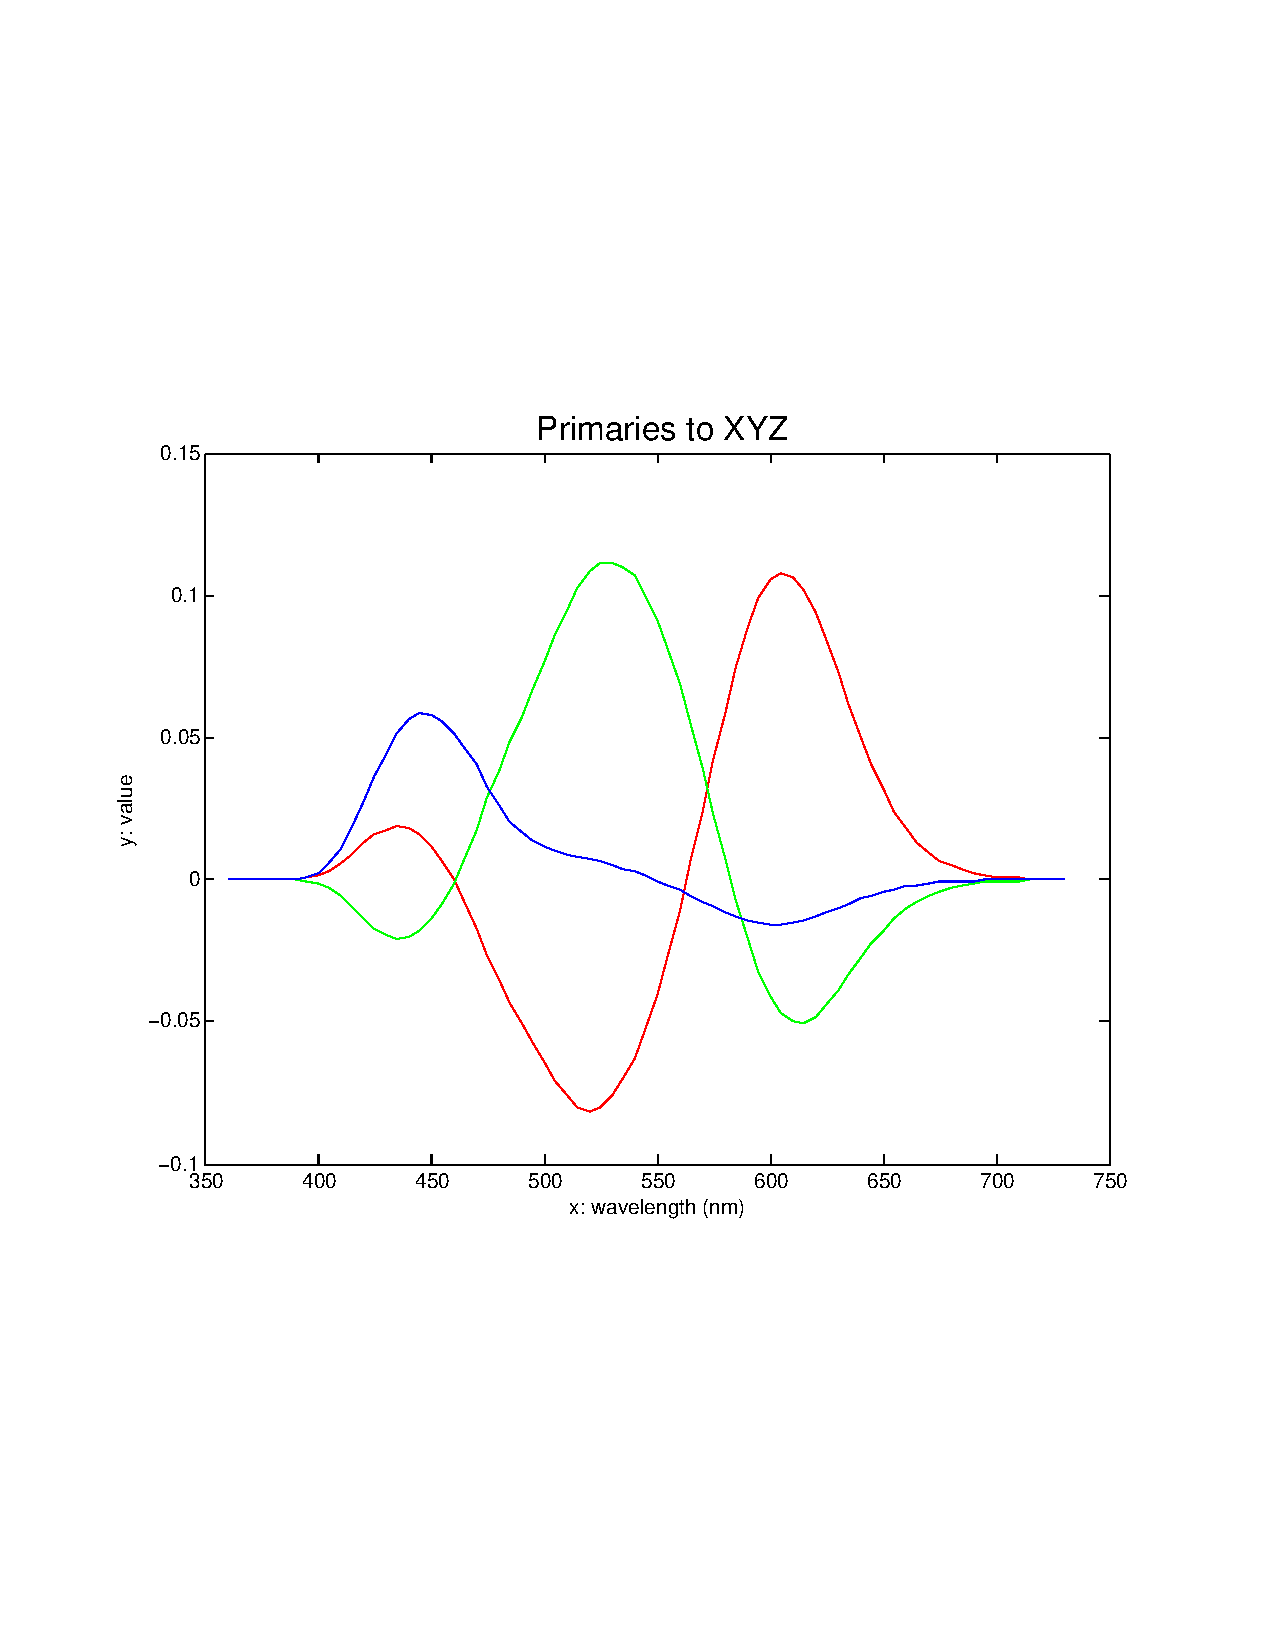
\includegraphics[width = 200pt, trim = 50pt 50pt 50pt 50pt, clip]{P_XYZ} \\
\end{tabular}

For both the RGB and XYZ spectras, the primaries have negative values in some areas because the color functions matrix $C$ is an underdetermined system with multiple solutions.  That is why we took the pseudoinverse rather than just the inverse.
\newline

\tabT \textbf{(b)} For the spectral response curves for the eye photreceptors, we find the primary light spectra again by taking the psuedoinverse of $LMSResponse$ matrix.  As a result we get the following primary light spectra.
\newline

\DeclareGraphicsExtensions{.pdf,.png,.jpg}
\tabT\tabT\tabT\tabT\tabT\tabT\tabT 
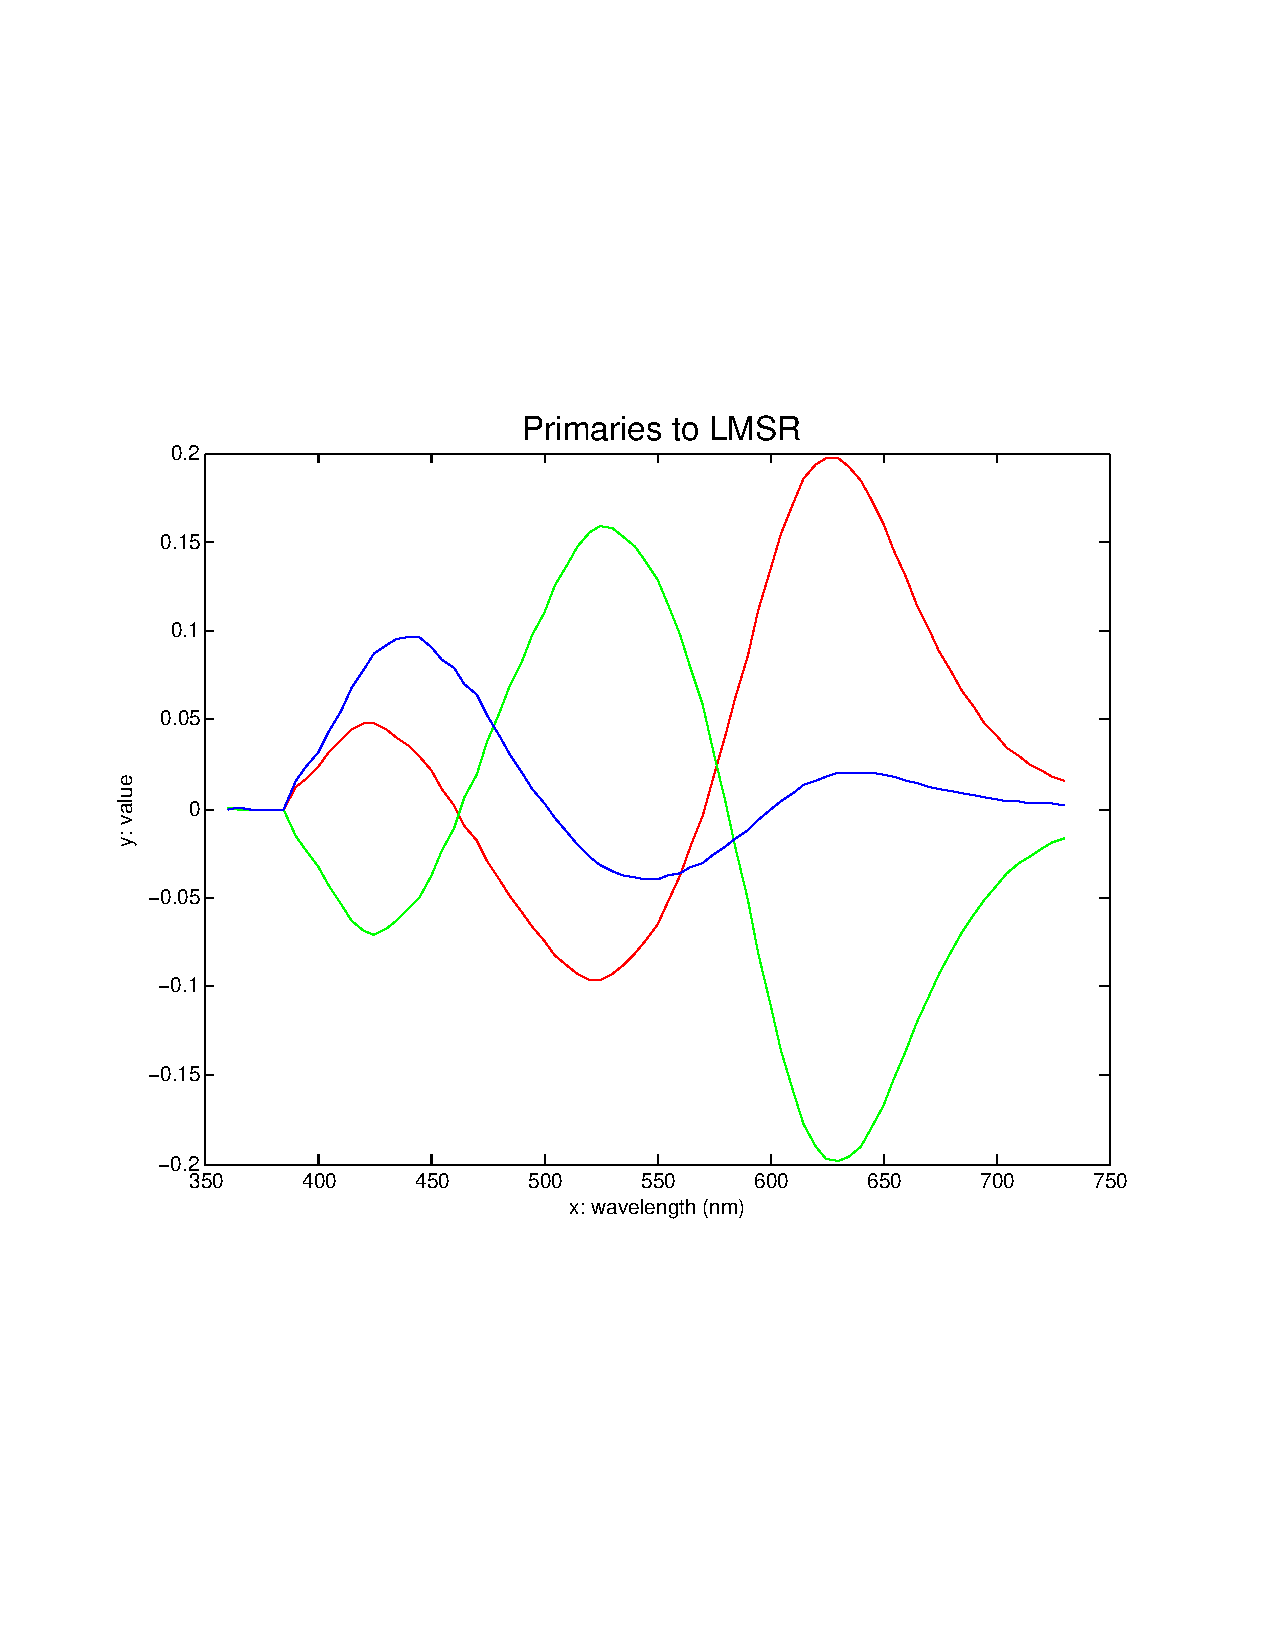
\includegraphics[width = 200pt, trim = 50pt 50pt 50pt 50pt, clip]{P_LMSR} 

By definition on the construction of this primary spectra, we can confirm that this is a valid set of primaries and satisfies Equation 1.  We notice that much of the spectrum has values that are very negative.
\newline

\tabT \textbf{(c)} If the spectral response curves of the eye (assumed to be non-negative) were orthogonal to each other (with a zero dot product), there would exist a corresponding set of primaries with power spectra that were non-negative.  This can be shown by the following.  Let $C_{LMSR}$ correspond to the spectral response composed of orthogonal columns.  Since the basis of this matrix is orthaganal to each other, $C_{LMSR}^{-1} = C_{LMSR}^{T}$.  This means that the power spectra to the LMSR is non-negative as well since it is the transpose of the spectral response matrix which is also non-negative. $P_{LMSR} = C_{LMSR}^{-1} = C_{LMSR}^{T}$. 
\newline


\section*{Problem 2}
\tabT \textbf{(A)} Below represents the a single layer neural network and the XOR dataset.  The sigmoid $\sigma(a)$ activation function has $0.5$ as the threshold (1 if $a \geq 0.5$, 0 if $a < 0.5$).
\newline
\newline

\begin{center}
\tabT\tabT\tabT\textbf{Single Layer Network}
\tabT\tabT\tabT \textbf{XOR dataset}
\newline
\DeclareGraphicsExtensions{.pdf,.png,.jpg}
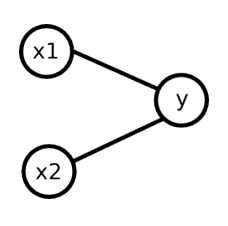
\includegraphics[width = 100pt]{XOR_singleL}
\tabT\tabT\tabT
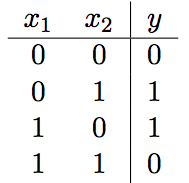
\includegraphics[width = 100pt]{XOR_logical}
\end{center}

\tabT A single layer network cannot classify the XOR dataset correctly because the data is not linearly separable.  You need at least two lines to separate the points (0,1)(1,0) from (0,0)(1,1).  This can be proven by examining the below constraints on the output node with all possible inputs.
\newline
\newline
$(0)w_{1} + (0)w_{2} < y$, \tabT\tabT $y > 0$ \newline
$(0)w_{1} + (1)w_{2} \geq y$, \tabT\tabT $w_{2} \geq 0.5$ \newline
$(1)w_{1} + (0)w_{2} \geq y$, \tabT\tabT $w_{1} \geq 0.5$ \newline
$(1)w_{1} + (1)w_{2} < y$, \tabT\tabT $w_{1} + w_{2} < 0.5$, \tabT\tabT
Contradiction: $0.5 + 0.5 \nless 0.5$ 
\newline
\newline
Last constraint fails and contradicts the prior constraints.  Since, at best, one classification fails out of the four, the best theoretical error is $.25$.
\newline

\textbf{(B)} Below represents the a hidden layer neural network for the XOR dataset.
\newline

\begin{center}
\tabT\tabT\tabT\tabT\tabT\textbf{Hidden Layer Network}
\newline
\DeclareGraphicsExtensions{.pdf,.png,.jpg}
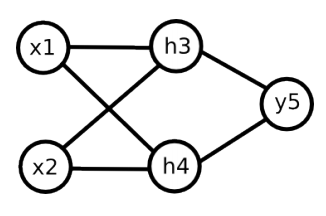
\includegraphics[width = 120pt]{XOR_hiddenL}
\end{center}
$a_{3} = w_{13}x_{1} + w_{23}x_{2} + b_{3}$, \tabT\tabT
$z_{3} = \sigma(a_{3})$, \tabT\tabT
$E = \frac{1}{2}(z_{5} - t)^2$
\newline
$a_{4} = w_{14}x_{1} + w_{24}x_{2} + b_{4}$, \tabT\tabT
$z_{4} = \sigma(a_{4})$, \tabT\tabT
$\sigma(x) = \frac{1}{1+e^{-x}}$
\newline
$a_{5} = w_{35}z_{3} + w_{45}z_{4} + b_{5}$, \tabT\tabT
$z_{5} = a_{5}$, \tabT\tabT\tabT
$\frac{\partial \sigma(x)}{\partial x} = \frac{e^x}{(1+e^{x})^2}$
\newline
\newline
\tabT\textbf{(i)} With the initialization that all weights $w_{ij} = 1$ and biases $b_{i} = 0$, calcuate the output and error using $(x_{1} = 0, x_{2} = 0)$.
\newline
\tabT \textbf{Output} $= z_{5} = a_{5} = w_{35}z_{3} + w_{45}z_{4} + b_{5}$
$= (1)\sigma(a_{3}) + (1)\sigma(a_{4}) = \frac{1}{1+e^{-0}} + \frac{1}{1+e^{-0}} = \frac{1}{2} + \frac{1}{2} = 1$
\newline
\tabT \textbf{Error} $= \delta_{5} = (z_{5} - t_{5}) = 1 - 0 = 1$
\newline
\newline
\tabT\textbf{(ii)} $\frac{\partial E}{\partial w_{35}} = \delta_{5}z_{3} = (z_{5} - t_{5})z_{3} = (1)z_{3} = \sigma(a_{3}) = \sigma(0) = \frac{1}{1+e^{-0}} = \frac{1}{2}$
\newline
\newline
\tabT\textbf{(iii)} $\frac{\partial E}{\partial w_{13}} = \delta_{3}z_{1} = (h'(a_{3})\sum_{k} w_{35}\delta_{k})x_{1} = \frac{e^x}{(1+e^{x})^2}w_{35}(z_{5}-t)x_{1} = \frac{1}{4}(1)(1)(0) = 0$
\newline
\newline
\tabT\textbf{(iv)} Show updated weights using $w_{ij} = w_{ij} - \eta\frac{\partial E}{\partial w_{ij}}$.  Below is the process of backpropogation, refer to last column of last table for updated weights after learning from $(x_{1} = 0, x_{2} = 1, y=1)$ and using $\eta = .1$
\newline
\newline
\begin{center}
  \begin{tabular}{ c | c | c }
    $node_{j}$ & $a_{j}$ & $z_{j}$ \\ \hline
    3 & 0+1=1 & $\frac{1}{1+e^{-1}} = .73$ \\
    4 & 0+1=1 & $\frac{1}{1+e^{-1}} = .73$ \\
    5 & .73+.73 = 1.46 & 1.46 \\
  \end{tabular}
\end{center}
\begin{center}
  \begin{tabular}{ c | c | c }
    $node_{j}$ & $\delta$ & $\delta_{j}$ \\ \hline
    5 & $z_{5}-t$ & 1.46-1 = .46 \\
    4 & $h'(a_{4})\sum_{k} w_{4k}\delta_{k} = \frac{e^{a_{4}}}{(1+e^{a_{4}})^2}w_{45}\delta_{5}$ & $\frac{e}{(1+e)^2}(1)(.46) = (.2)(.46) = .09$ \\
    3 & $h'(a_{3})\sum_{k} w_{3k}\delta_{k} = \frac{e^{a_{3}}}{(1+e^{a_{3}})^2}w_{35}\delta_{5}$ & $\frac{e}{(1+e)^2}(1)(.46) = (.2)(.46) = .09$ \\
  \end{tabular}
\end{center}
\begin{center}
  \begin{tabular}{ c | c | c }
    $node_{ij}$ & $gradient$ & $\frac{\partial E}{\partial w_{ij}}$ \\ \hline
    35 & $z_{3}\delta_{5}$ & .73(.46) = .34 \\
    45 & $z_{4}\delta_{5}$ & .73(.46) = .34 \\
    13 & $z_{1}\delta_{3}$ & 0(.09) = 0 \\
    14 & $z_{1}\delta_{4}$ & 0(.09) = 0 \\
    23 & $z_{2}\delta_{3}$ & 1(.09) = .09 \\
    24 & $z_{2}\delta_{4}$ & 1(.09) = .09 \\
  \end{tabular}
\end{center}
\begin{center}
  \begin{tabular}{ c | c | c }
    $w_{ij}$ & $w_{ij}^{-} - \eta\frac{\partial E}{\partial w_{ij}}$ & $w_{ij}^{+}$ \\ \hline
    35 & 1-(.1)(.34) & .97 \\
    45 & 1-(.1)(.34) & .97 \\
    13 & 1-(.1)(0) & 1 \\
    14 & 1-(.1)(0) & 1 \\
    23 & 1-(.1)(.09) & .991 \\
    24 & 1-(.1)(.09) & .991 \\
  \end{tabular}
\end{center}

\textbf{(C)} Backpropagation is \textbf{not} gauranteed to find the optimal solution.  According to \textit{Back Propagation is Sensitive to Initial Conditions} by Kolen and Pollack, the algorithm is a heuristic that will find a local optimum but not necessarily the global optimum.  It is the initial weights that decides which local optimum it will find and no overall seach can be done to find the optimal set of weights.  Therefore, backpropagation depends on the training set and initial conditions, which may not necessarily find the best solution. 

\end{document}
